\section{Problem description}
% \subsection{Dominant patterns}
\begin{figure}
\begin{center}
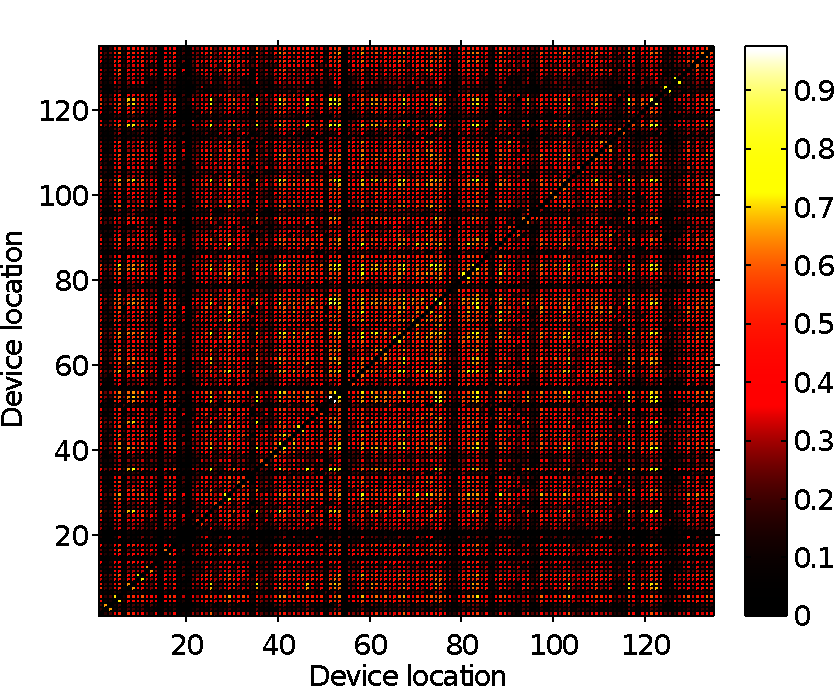
\includegraphics[width=.5\textwidth]{img/heatMap_raw_201106-eps-converted-to.pdf}
\caption{Correlation coefficients of the raw traces from the Building 1 dataset (Section \ref{data:engbldg2}).
The matrix is ordered such as the devices serving same/adjacent rooms are nearby in the matrix.}
\label{fig:heatmap:raw}
\end{center}
\end{figure}

%The first step of the proposed approach is to uncover from the raw data the devices that are used all together.
The primary objective of SBS is to determine the devices that are used simulataneously.
%The basic tool that allows us to compare device energy consumption is the correlation coefficient.
Classical approaches would run correlation analyses across pairs of power-draw signals between distinct devices, summarized by a correlation coefficient.  
However, doing that does not yield any useful information when applied to the raw data.
%However, during our experiments we found that it provides poor help when it is directly applied to the raw signals.
For example the two raw signals of Figure \ref{fig:diagram1} are from two independent HVAC systems serving different rooms on different floors.
Since each space is independently controlled, we expect their power-draw signals to be uncorrelated (or at least distinguishable 
from other signal pairs).  However, their correlation coefficient ($0.57$) was not particularly informative.  
% however, their correlation coefficient (i.e. $0.5675$) indicates the opposite.
%Another example, with 135 devices, is depicted in Figure \ref{fig:heatmap:raw}.

% Another example, depicted in Figure \ref{fig:heatmap:raw}, shows a correlation matrix with 135 distinct locations, each containing a number of devices.  
Using a larger set of devices, Figure \ref{fig:heatmap:raw} shows a correlation matrix with 135 distinct lighting and HVAC systems serving numerous rooms in a building (described later on in Section \ref{data:engbldg2}).
The indices are selected such that their index-difference is indicative of their relative spatial proximity.  
For example, a device in location 1 is closer in the building to a device in location 2 than it is to 
a device in location 135. 
% We do not account for obstructions between them, such as walls.  %?
The color of the cell is the average pairwise correlation coefficient for devices in the row-column index.  The higher the value, the lighter the color.
%the devices serving the same (or adjacent) room are close
%to one another in the matrix.  
Devices serving the same room are along the diagonal.  Because these devices are used simultaneously, we expect
high average correlation scores, lighter shades, along the diagonal figure.
%and because they are used simultaneously by the room users we expect them to feature the highest correlation scores.
However, we observe no such pattern.  %structure is unseen in the Figure.  
Most of the signals are correlated with all the others and we see no discernable structure.
% thus this metric prevents us from finding devices that are used in concert.

\begin{figure}[t!]
\begin{center}
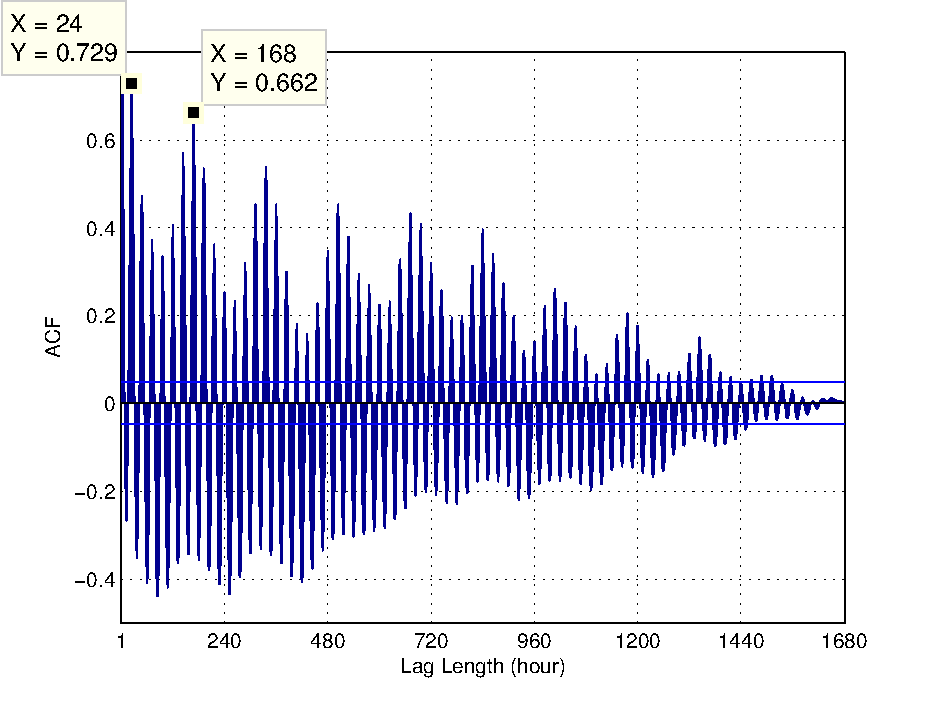
\includegraphics[width=.5\textwidth]{img/acf_101A1_GHP-eps-converted-to.pdf}
\caption{Auto-correlation of a usual signal from the Building 1 dataset.
The signal features daily and weekly patterns (resp. $x=24$ and $x=168$).}
\label{fig:autocorr}
\end{center}
\end{figure}

An explanation for this is that the daily occupant usage patterns %office hours, 
drive these results.
Figure \ref{fig:diagram1} demonstrates this more clearly.  It shows two 1-week raw signals traces which feature the same 
diurnal pattern.  
This trend is present in almost every sensor trace, and, it hides 
the smaller fluctuations providing more specific patterns driven by local occupant activity.  Upon deeper inspection, we uncovered several
 dominant patterns, common among energy-consuming devices in buildings~\cite{wrinch:pes2012}.  Figure~\ref{fig:autocorr} depicts the 
 auto-correlation of a usual electric power signal for a device.  The two highest values in the figure correspond to a lag of 24 hours and 168 hours (one week).  
 Therefore, the signal has some periodicity and similar (though not equal) values are seen at daily and weekly time scales.
The daily pattern is due to daily office hours and the weekly pattern corresponds to weekdays and weekends.  
%Indeed, thorough inspection of the data reveals that the 
Clearly, the use of correlation analysis on the \emph{raw} signals cannot be used to determine meaningful 
inter-device relationships because periodic components act as non-stationary trends for quicker phenomenon, hence making correlation functions irrelevant.  %metric is insufficient with raw signals containing the same dominant pattern.

Such trends must be removed in order to make meaningful progress towards our aforementioned goals.  In the next section
we describe SBS.  We discuss \emph{strip and bind} in section~\ref{methodo:est}, which addresses the detrending and
relationship-discovery challenge.  Then we describe how we \emph{search} for changes in those usage patterns, 
in section~\ref{methodo:ano}, to identify potential opportunities for savings.

%One of the major challenges in this work is to discard these patterns and uncover devices intrinsic relationships.
% This difficulty is overcome by the first part of the method (Strip and Bind) presented in Section \ref{methodo:est}.
% Then, the second part of the method (Search) monitors over time the devices relationships and detect abnormal device behavior changes (Section \ref{methodo:ano}).
